\documentclass[11pt,compress,t,notes=noshow, xcolor=table]{beamer}
\usepackage[]{graphicx}\usepackage[]{color}
% maxwidth is the original width if it is less than linewidth
% otherwise use linewidth (to make sure the graphics do not exceed the margin)
\makeatletter
\def\maxwidth{ %
  \ifdim\Gin@nat@width>\linewidth
    \linewidth
  \else
    \Gin@nat@width
  \fi
}
\makeatother

\newcommand{\citebutton}[2]{%
\beamergotobutton{\href{#2}{#1}}%
}

\newcommand{\blu}[1]{\textcolor{blue}{#1}}
\newcommand{\org}[1]{\textcolor{orange}{#1}}
\newcommand{\ques}{\textbf{\textcolor{red}{Question:  }}}
\newcommand{\questionssofar}{\begin{frame}\frametitle{Any questions?}\end{frame}}

\newcommand\warning{%
 \makebox[1.4em][c]{%
 \makebox[0pt][c]{\raisebox{.1em}{\scriptsize!}}%
 \makebox[0pt][c]{\color{red}\normalsize$\bigtriangleup$}}}%

\definecolor{fgcolor}{rgb}{0.345, 0.345, 0.345}
\newcommand{\hlnum}[1]{\textcolor[rgb]{0.686,0.059,0.569}{#1}}%
\newcommand{\hlstr}[1]{\textcolor[rgb]{0.192,0.494,0.8}{#1}}%
\newcommand{\hlcom}[1]{\textcolor[rgb]{0.678,0.584,0.686}{\textit{#1}}}%
\newcommand{\hlopt}[1]{\textcolor[rgb]{0,0,0}{#1}}%
\newcommand{\hlstd}[1]{\textcolor[rgb]{0.345,0.345,0.345}{#1}}%
\newcommand{\hlkwa}[1]{\textcolor[rgb]{0.161,0.373,0.58}{\textbf{#1}}}%
\newcommand{\hlkwb}[1]{\textcolor[rgb]{0.69,0.353,0.396}{#1}}%
\newcommand{\hlkwc}[1]{\textcolor[rgb]{0.333,0.667,0.333}{#1}}%
\newcommand{\hlkwd}[1]{\textcolor[rgb]{0.737,0.353,0.396}{\textbf{#1}}}%
\let\hlipl\hlkwb

\usepackage{framed}
\makeatletter
\newenvironment{kframe}{%
 \def\at@end@of@kframe{}%
 \ifinner\ifhmode%
  \def\at@end@of@kframe{\end{minipage}}%
  \begin{minipage}{\columnwidth}%
 \fi\fi%
 \def\FrameCommand##1{\hskip\@totalleftmargin \hskip-\fboxsep
 \colorbox{shadecolor}{##1}\hskip-\fboxsep
     % There is no \\@totalrightmargin, so:
     \hskip-\linewidth \hskip-\@totalleftmargin \hskip\columnwidth}%
 \MakeFramed {\advance\hsize-\width
   \@totalleftmargin\z@ \linewidth\hsize
   \@setminipage}}%
 {\par\unskip\endMakeFramed%
 \at@end@of@kframe}
\makeatother

\definecolor{shadecolor}{rgb}{.97, .97, .97}
\definecolor{messagecolor}{rgb}{0, 0, 0}
\definecolor{warningcolor}{rgb}{1, 0, 1}
\definecolor{errorcolor}{rgb}{1, 0, 0}
\newenvironment{knitrout}{}{} % an empty environment to be redefined in TeX

\usepackage{alltt}
\newcommand{\SweaveOpts}[1]{}  % do not interfere with LaTeX
\newcommand{\SweaveInput}[1]{} % because they are not real TeX commands
\newcommand{\Sexpr}[1]{}       % will only be parsed by R
\newcommand{\xmark}{\ding{55}}%


\usepackage[english]{babel}
\usepackage[utf8]{inputenc}

\usepackage{dsfont}
\usepackage{verbatim}
\usepackage{amsmath}
\usepackage{amsfonts}
\usepackage{amssymb}
\usepackage{bm}
\usepackage{csquotes}
\usepackage{multirow}
\usepackage{longtable}
\usepackage{booktabs}
\usepackage{enumerate}
\usepackage[absolute,overlay]{textpos}
\usepackage{psfrag}
\usepackage{algorithm}
\usepackage{algpseudocode}
\usepackage{eqnarray}
\usepackage{arydshln}
\usepackage{tabularx}
\usepackage{placeins}
\usepackage{tikz}
\usepackage{setspace}
\usepackage{colortbl}
\usepackage{mathtools}
\usepackage{wrapfig}
\usepackage{bm}
\usepackage{amsmath}
\usepackage{pifont}

\usetikzlibrary{shapes.multipart,shapes,arrows,automata,positioning,calc,chains,trees, shadows}
\tikzset{
  %Define standard arrow tip
  >=stealth',
  %Define style for boxes
  punkt/.style={
    rectangle,
    rounded corners,
    draw=black, very thick,
    text width=6.5em,
    minimum height=2em,
    text centered},
  % Define arrow style
  pil/.style={
    ->,
    thick,
    shorten <=2pt,
    shorten >=2pt,}
}

\tikzstyle{vec}=[draw, rectangle, fill = white, minimum width=5mm, minimum height=1cm, inner sep = 2pt]

\usepackage{subfig}

% Defines macros and environments
\usepackage{../../style/lmu-lecture}


\let\code=\texttt
\let\proglang=\textsf

\setkeys{Gin}{width=0.9\textwidth}

\setbeamertemplate{frametitle}{\expandafter\uppercase\expandafter\insertframetitle}

\usepackage{bbm}
% basic latex stuff
\newcommand{\pkg}[1]{{\fontseries{b}\selectfont #1}} %fontstyle for R packages
\newcommand{\lz}{\vspace{0.5cm}} %vertical space
\newcommand{\dlz}{\vspace{1cm}} %double vertical space
\newcommand{\oneliner}[1] % Oneliner for important statements
{\begin{block}{}\begin{center}\begin{Large}#1\end{Large}\end{center}\end{block}}


%new environments
\newenvironment{vbframe}  %frame with breaks and verbatim
{
 \begin{frame}[containsverbatim,allowframebreaks]
}
{
\end{frame}
}

\newenvironment{vframe}  %frame with verbatim without breaks (to avoid numbering one slided frames)
{
 \begin{frame}[containsverbatim]
}
{
\end{frame}
}

\newenvironment{blocki}[1]   % itemize block
{
 \begin{block}{#1}\begin{itemize}
}
{
\end{itemize}\end{block}
}

\newenvironment{fragileframe}[2]{  %fragile frame with framebreaks
\begin{frame}[allowframebreaks, fragile, environment = fragileframe]
\frametitle{#1}
#2}
{\end{frame}}


\newcommand{\myframe}[2]{  %short for frame with framebreaks
\begin{frame}[allowframebreaks]
\frametitle{#1}
#2
\end{frame}}

\newcommand{\remark}[1]{
  \textbf{Remark:} #1
}


\newenvironment{deleteframe}
{
\begingroup
\usebackgroundtemplate{
\includegraphics[width=\paperwidth,height=\paperheight]{../style/color/red.png}}
 \begin{frame}
}
{
\end{frame}
\endgroup
}
\newenvironment{simplifyframe}
{
\begingroup
\usebackgroundtemplate{
\includegraphics[width=\paperwidth,height=\paperheight]{../style/color/yellow.png}}
 \begin{frame}
}
{
\end{frame}
\endgroup
}\newenvironment{draftframe}
{
\begingroup
\usebackgroundtemplate{
\includegraphics[width=\paperwidth,height=\paperheight]{../style/color/green.jpg}}
 \begin{frame}
}
{
\end{frame}
\endgroup
}
% https://tex.stackexchange.com/a/261480: textcolor that works in mathmode
\makeatletter
\renewcommand*{\@textcolor}[3]{%
  \protect\leavevmode
  \begingroup
    \color#1{#2}#3%
  \endgroup
}
\makeatother





\input{../../latex-math/basic-math.tex}
\input{../../latex-math/basic-ml.tex}

\newcommand{\titlefigure}{figure/linear-relationships.png}
\newcommand{\learninggoals}{
\item Understand what word embeddigns are
\item Learn the main methods for creating them}

\title{Basics}
% \author{}
\institute{\href{https://slds-lmu.github.io/lecture_dl4nlp/}{slds-lmu.github.io/lecture\_dl4nlp}}
\date{}

\begin{document}
\lecturechapter{Word Embeddings}
\lecture{Deep Learning for NLP}

% ------------------------------------------------------------------------------

\begin{vbframe}{Motivation (1)}

\vfill

\begin{itemize}
	\item How to represent words/tokens in a neural network?
	\item Possible solution: one-hot encoded indicator vectors of length $|V|$.
\end{itemize}

\begin{center}
\begin{minipage}{.2\textwidth}
	\[\vec w^{({\text{the}})} =
	\begin{bmatrix}
	1 \\ 0 \\ 0 \\ \vdots
	\end{bmatrix}
	\]
\end{minipage}
\begin{minipage}{.2\textwidth}
	\[\vec w^{({\text{cat}})} =
	\begin{bmatrix}
	0 \\ 1 \\ 0 \\ \vdots
	\end{bmatrix}
	\]
\end{minipage}
\begin{minipage}{.2\textwidth}
\[\vec w^{({\text{dog}})} =
\begin{bmatrix}
0 \\ 0 \\ 1 \\ \vdots
\end{bmatrix}
\]
\end{minipage}
\end{center}

\begin{itemize}
	\item \ques Why is this a bad idea?
		\begin{itemize}
			\item Parameter explosion ($|V|$ might be $> 1M$)
			\item All word vectors are orthogonal to each other\\$\rightarrow$ no notion of word similarity
		\end{itemize}
\end{itemize}

\vfill

\end{vbframe}

% ------------------------------------------------------------------------------

\begin{vbframe}{Motivation (2)}

\vfill

\begin{itemize}
	\item Learn one word vector $\vec w^{(i)} \in \mathbb{R}^{D}$ (``word embedding'') per word $i$
	\item Typical dimensionality: $50 \leq D \leq 1000 \ll |V|$
	\item Embedding matrix: $\mathbf{W} \in \mathbb{R}^{|V|\times D}$
	\item \ques Advantages of using word vectors?
		\begin{itemize}
			\item We can express similarities between words, e.g., with cosine similarity:
		\end{itemize}
		 $$\mathrm{cos}(\vec w^{(i)}, \vec w^{(j)}) = \frac{\mathbf{w}^{(i)T}\mathbf{w}^{(j)}}{\lVert \mathbf{w}^{(i)} \rVert_2 \cdot \lVert \mathbf{w}^{(j)}\lVert_2}$$
		\begin{itemize}
			\item Since the embedding operation is a \emph{lookup operation}, we only need to update the vectors that occur in a given training batch
		\end{itemize}
\end{itemize}

\vfill

\end{vbframe}

% ------------------------------------------------------------------------------

\begin{vbframe}{Motivation (3)}

\vfill

\textbf{Supervised training?}

\begin{itemize}
	\item \textit{Training from scratch}:
	\\ $\rightarrow$ Initialize embeddings randomly and learn it during training phase
	\\ $\rightarrow$ Words that play similar roles w.r.t. task get similar embeddings
	\item \textit{From sentiment classification}: 
	\\ $\rightarrow$ We might expect $\vec w^{(\text{great})} \approx \vec w^{(\text{awesome})}$
	\item \ques What could be a problem at test time?
	\begin{itemize}
		\item If training set is small, many words are unseen during training and therefore have random vectors
	\end{itemize}
	\item We typically have more unlabeled than labeled data.
	\\ $\rightarrow$ Can we learn embeddings from the unlabeled data?
\end{itemize}

\vfill

\end{vbframe}

% ------------------------------------------------------------------------------

\begin{vbframe}{Motivation (4)}

\vfill

\begin{itemize}
	\item Distributional hypothesis: 
	\\ {\centering ``\textit{A word is characterized by the company it keeps}``}
	\\ {\centering (J.R. Firth, 1957)}
	\item Idea: Learn similar vectors for words that occur in similar contexts
	\item Three different (milestone) methods:
		\begin{itemize}
			\item Word2Vec \beamergotobutton{\href{https://arxiv.org/abs/1301.3781}{(Mikolov et al., 2013)}}
			\item GloVe (not covered) \beamergotobutton{\href{https://aclanthology.org/D14-1162/}{(Pennington et al., 2014)}}
			\item FastText \beamergotobutton{\href{https://arxiv.org/abs/1607.04606}{(Bojanowski et al., 2016)}}
		\end{itemize}
\end{itemize}

\vfill

\end{vbframe}

% ------------------------------------------------------------------------------

%\begin{vbframe}{again: language models}

%\vfill

%\begin{itemize}
%	\item \ques What is a Language Model?
%		\begin{itemize}
%			\item Function to assign probability to a sequence of words.
%		\end{itemize}
%	\item \ques What is an n-gram language Model?
%		\begin{itemize}
%			\item Markov assumption: probability of word only depends on no more than $n-1$ other (previous) words:
%			$$P(w_{[1]} \dots w_{[T]}) = \prod_{t=1}^T P(w_{[t]}|w_{[t-1]} ... w_{[t - n + 1]}) $$
%		\end{itemize}
%\end{itemize}

%\vfill

%\end{vbframe}

% ------------------------------------------------------------------------------

\begin{vbframe}{Word2Vec as a Bigram Language Model}

\vfill

\begin{itemize}
	\item Words in our vocabulary are represented as two sets of vectors:
		\begin{itemize}
			 \item $\vec w^{(i)} \in \mathbb{R}^D$ if they are to be predicted
			 \item $\vec v^{(i)} \in \mathbb{R}^D$ if they are conditioned on as context
		\end{itemize}
	\item Predict word $i$ given previous word $j$: $$P(i|j) = f(\vec w^{(i)}, \vec v^{(j)})$$
	\item \ques What is a possible function $f(\cdot)$ ?
\end{itemize}

\vfill

\end{vbframe}

% ------------------------------------------------------------------------------

\begin{vbframe}{A Simple Neural Network Bigram Language Model}

\vfill

\begin{itemize}
	\item Softmax!
	$$P(i|j) = \frac{exp(\mathbf{w}^{(i)T} \mathbf{v}^{(j)})}{\sum_{k=1}^{|V|} exp(\mathbf{w}^{(k)T} \mathbf{v}^{(j)})}$$
	\item[]
	\item \ques Problem with training softmax?
	\\ $\rightarrow$ \textit{SLOW}
	\\ (Needs to compute dot products with the whole vocabulary in the denominator for every single prediction)
\end{itemize}

\vfill

\end{vbframe}

% ------------------------------------------------------------------------------

\begin{vbframe}{Hierarchical Softmax}

\vfill

\begin{itemize}
	\item Context vectors $\vec v$ are defined like before.
	\item Word vectors $\vec w$ are replaced by a binary tree:
\end{itemize}

\begin{center}
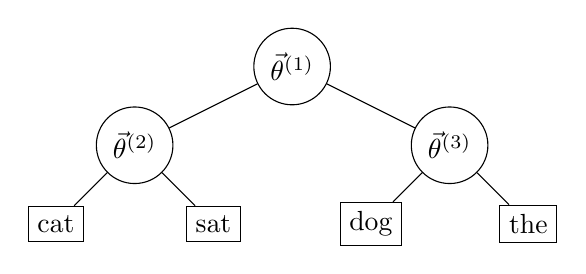
\begin{tikzpicture}
\node (root) [draw, circle] at (0,0) {$\vec \theta^{(1)}$};
\node (theta1) [draw, circle] at (-2,-1) {$\vec \theta^{(2)}$};
\node (theta2) [draw, circle] at (2,-1) {$\vec \theta^{(3)}$};
\draw (root) -- (theta1);
\draw (root) -- (theta2);
\node (w1) [draw, rectangle] at (-3,-2) {cat};
\node (w2) [draw, rectangle] at (-1,-2) {sat};
\node (w3) [draw, rectangle] at (1,-2) {dog};
\node (w4) [draw, rectangle] at (3,-2) {the};
\draw (theta1) -- (w1);
\draw (theta1) -- (w2);
\draw (theta2) -- (w3);
\draw (theta2) -- (w4);
\end{tikzpicture}
\end{center}

\vfill

\end{vbframe}

% ------------------------------------------------------------------------------

\begin{vbframe}{Hierarchical Softmax}

\vfill

\begin{itemize}
 \item Each tree node $l$ has parameter vector $\vec \theta^{(l)}$
 \item Probability of going left at node $l$ given context word $j$: $p(\text{left}|l,j) = \sigma(({\vec {\theta}}^{(l)})^T ~\vec v^{(j)})$
 \item Probability of going right: $p(\text{right}|l,j) = 1-p(\text{left}|l,j)$
 \item Probability of word $i$ given $j$: product of probabilities on the path from root to $i$
\end{itemize}

\vfill

\end{vbframe}

% ------------------------------------------------------------------------------

\begin{vbframe}{Example}

\vfill

Calculate $p(\text{sat}|\text{cat})$.

\begin{center}
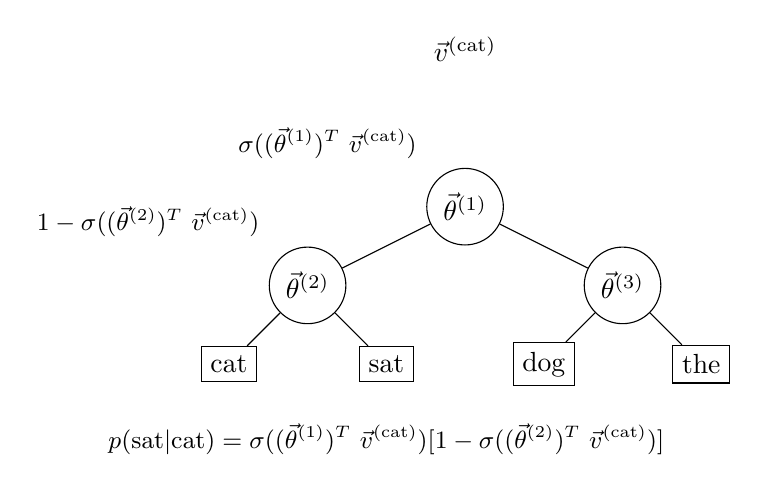
\begin{tikzpicture}
\node (v) at (0,2) {$\vec v^{(\text{cat})}$};
\node (root) [draw, circle] at (0,0) {$\vec \theta^{(1)}$};
\node (theta1) [draw, circle] at (-2,-1) {$\vec \theta^{(2)}$};
\node (theta2) [draw, circle] at (2,-1) {$\vec \theta^{(3)}$};
\draw (root) -- (theta1);
\draw (root) -- (theta2);
\node (w1) [draw, rectangle] at (-3,-2) {cat};
\node (w2) [draw, rectangle] at (-1,-2) {sat};
\node (w3) [draw, rectangle] at (1,-2) {dog};
\node (w4) [draw, rectangle] at (3,-2) {the};
\draw (theta1) -- (w1);
\draw (theta1) -- (w2);
\draw (theta2) -- (w3);
\draw (theta2) -- (w4);

\node [above left=2mm of root] {\small $\sigma((\vec \theta^{(1)})^T ~\vec v^{(\text{cat})})$};

\node [above left=2mm of theta1] {\small $1-\sigma((\vec \theta^{(2)})^T ~\vec v^{(\text{cat})})$};

\node [below=4mm of w2] {\small $p(\text{sat}|\text{cat}) = \sigma((\vec \theta^{(1)})^T ~\vec v^{(\text{cat})}) [1-\sigma((\vec \theta^{(2)})^T ~\vec v^{(\text{cat})})]$};
\end{tikzpicture}
\end{center}

\vfill

\end{vbframe}

% ------------------------------------------------------------------------------

\begin{vbframe}{Questions}

\vfill

\begin{itemize}
	\item \ques How many dot products do we need to calculate to get to $p(i|j)$? How does this compare to the naive softmax?
		\begin{itemize}
			\item $\log_2|V| \ll |V|$
		\end{itemize}
	\vskip5mm
	\item \ques Show that $\sum_{i'} p(i'|j)$ sums to 1.
\end{itemize}

\vfill

\end{vbframe}

% ------------------------------------------------------------------------------

\begin{vbframe}{Speeding up Training: Negative Sampling}

\vfill

\begin{itemize}
	\item Another trick: \textbf{negative sampling}\\ (a variant of \emph{noise contrastive estimation})
	\item This changes the objective function, and the resulting model is not a language model anymore!
	\item \textbf{Idea}: Instead of predicting the probability distribution over whole vocabulary, make binary decisions for a small number of words.
	\item ``Positive`` samples: Bigrams seen in the corpus.
	\item ``Negative`` samples: Random bigrams (not seen in the corpus).
\end{itemize}

\vfill

\end{vbframe}

% ------------------------------------------------------------------------------

\begin{vbframe}{Negative Sampling: Likelihood}

\vfill

\begin{itemize}
	\item Given:
		\begin{itemize}
			\item Positive training set: $\mathrm{pos}(\mathcal{O})$
			\item Negative training set: $\mathrm{neg}(\mathcal{O})$
		\end{itemize}
\end{itemize}

	$$ L = \prod_{(i,j) \in \mathrm{pos}(\mathcal{O})} P(\mathrm{pos}|\vec w^{(i)}, \vec v^{(j)}) \prod_{(i',j') \in \mathrm{neg}(\mathcal{O})} P(\mathrm{neg}|\vec w^{(i')},\vec v^{(j')} ) $$
	
\begin{itemize}
	\item $P(\mathrm{pos}|\vec w, \vec v) = \sigma(\vec w^T \vec v)$
	\item $P(\mathrm{neg}|\vec w, \vec v) = 1-P(\mathrm{pos}|\vec w, \vec v)$
	\item \ques Why not just maximize $\displaystyle \prod_{(i,j) \in \mathrm{pos}(\mathcal{O})} P(\mathrm{pos}|\vec w^{(i)}, \vec v^{(j)}) $?
		\begin{itemize}
		\item Trivial solution: make all $\vec w, \vec v$ identical
		\end{itemize}
\end{itemize}

\vfill

\end{vbframe}

% ------------------------------------------------------------------------------

\begin{vbframe}{Word2Vec with negative sampling as classification}

\vfill

\begin{itemize}
	\item Maximize likelihood of training data:
	$$\mathcal{L}(\theta) = \prod_{i} P(y^{(i)}|x^{(i)}; \theta)$$
	\item $\Leftrightarrow$ minimize negative log likelihood:
	$$NLL(\theta) = - \log \mathcal{L}(\theta) = - \sum_{i} \log P(y^{(i)}|x^{(i)}; \theta))$$
	\item \ques What do these components stand for in Word2Vec with negative sampling?
		\begin{itemize}
			\item $x^{(i)}$ Word pair, from corpus OR randomly created
			\item $y^{(i)}$ Label: $1 = $ word pair is from positive training set, $0 = $ word pair is from negative training set
			\item $\theta$ Parameters $\vec v$, $\vec w$
			\item $P(...)$ Logistic sigmoid: $P(1|\cdot) = \sigma(\vec w^T \vec v)$, resp. $P(0|\cdot) = 1-\sigma(\vec w^T \vec v)$.
		\end{itemize}
\end{itemize}

\vfill

\end{vbframe}

% ------------------------------------------------------------------------------

\begin{vbframe}{Speeding up Training: Negative Sampling}

\vfill

\begin{itemize}
	\item Constructing a good negative training set can be difficult
	\item Often it is some random perturbation of the training data (e.g. replacing the second word of each bigram by a random word).
	\item The number of negative samples is often a multiple (1x to 20x) of the number of posisive samples
	\item Negative sets are often constructed per batch
\end{itemize}

\vfill

\end{vbframe}

% ------------------------------------------------------------------------------

\begin{vbframe}{Questions}

\vfill

\begin{itemize}
	\item \ques How many dot products do we need to calculate for a given word pair? How does this compare to the naive and hierarchical softmax?
		\begin{itemize}
			\item $M+1 \approx \mathrm{log}_2 |V| \ll |V|$
			\item (for $M=20, |V| = 1,000,000$)
		\end{itemize}
\end{itemize}

\vfill

\end{vbframe}

% ------------------------------------------------------------------------------

\begin{vbframe}{Skip-gram (Word2Vec)}

\vfill

\begin{minipage}{.63\textwidth}
\begin{itemize}
	\item Idea: Learn many bigram language models at the same time.
	\item Given word $w_{[t]}$, predict words inside a window around $w_{[t]}$:
		\begin{itemize}
			 \item One position before the target word: $p(w_{[t-1]}|w_{[t]})$
			 \item One position after the target word: $p(w_{[t+1]}|w_{[t]})$
			 \item Two positions before the target word: $p(w_{[t-2]}|w_{[t]})$
			 \item ... up to a specified window size $c$.
		\end{itemize}
	\item Models share all $\vec w$, $\vec v$ parameters!
\end{itemize}
\end{minipage}
\begin{minipage}{.36\textwidth}
\begin{center}
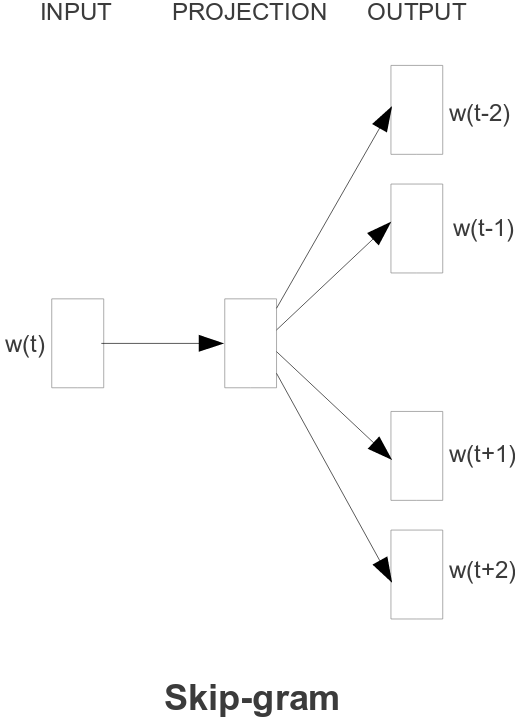
\includegraphics[scale=0.99]{figure/skipgram}
\end{center}
\end{minipage}

\vfill

\end{vbframe}

% ------------------------------------------------------------------------------

\begin{vbframe}{Skip-gram: Objective}

\vfill

\footnotesize
\begin{itemize}
	\item Optimize the joint likelihood of the $2c$ language models:
	$$p (w_{[t-c]} \dots w_{[t-1]} w_{[t+1]} \dots w_{[t+c]}|w_{[t]}) = \prod_{\substack{i \in  \{-c \ldots c\}\\ i \neq 0}} p(w_{[t+i]}|w_{[t]})$$
	
	\item Negative Log-likelihood for whole corpus (of size $N$):
	
	$$NLL = - \sum_{t=1}^N \sum_{\substack{i \in  \{-c \ldots c\}\\ i \neq 0}} \log p (w_{[t+i]}|w_{[t]})$$

	\item Using negative sampling as approximation:
		$$\approx - \sum_{t=1}^N \sum_{\substack{i \in  \{-c \ldots c\}\\ i \neq 0}} \Big[ \log \sigma(\vec w_{[t+i]}^T \vec v_{[t]}) + \sum_{m=1}^{M} \log [1-\sigma(\vec w^{{(*)}^T} \vec v_{[t]})]\Big] $$
	\item $\vec w^{(*)}$ is the word vector of a random word, $M$ is the number of negatives per positive sample
\end{itemize}

\vfill

\end{vbframe}

% ------------------------------------------------------------------------------

\begin{vbframe}{C(ontinuous) B(ag) o(f) W(ords)}

\vfill

\begin{minipage}{.58\textwidth}
\begin{itemize}
	\item Like Skipgram, but...
	\item Predict word $w_{[t]}$, given the words inside the window around $w_{[t]}$:
	 $$p(w_{[t]}|w_{[t-c]} \ldots w_{[t-1]} w_{[t+1]} \ldots w_{[t+c]})$$
	 $$\propto \vec w_{[t]}^T \sum_{\substack{i \in {-c\ldots c} \\ i \neq 0}} \vec v_{[t+i]}$$
\end{itemize}
\end{minipage}
\begin{minipage}{.41\textwidth}
\begin{center}
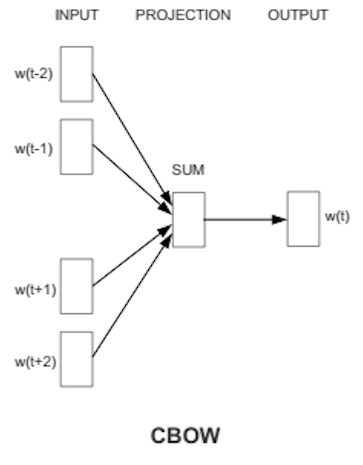
\includegraphics[scale=0.99]{figure/cbow}
\end{center}
\end{minipage}

\vfill

\end{vbframe}

% ------------------------------------------------------------------------------

%\begin{vbframe}{CBOW Command Example}

%\vfill

%\begin{verbatim}
%$ word2vec -train data.txt -output vec.txt -window 5 
%  -negative 20 -hs 0 -cbow 1
%\end{verbatim}

%\vfill

%\end{vbframe}

% ------------------------------------------------------------------------------

\begin{vbframe}{FastText (1)}

\vfill

\begin{itemize}
	\item Even if we train Word2Vec on a very large corpus, we will still encounter unknown words at test time
	\item Orthography can often help us:
	\item $\vec w^{(\text{remuneration})}$ should be similar to
		\begin{itemize}
			\item $\vec w^{(\text{remunerate})}$ (same stem)
			\item $\vec w^{(\text{iteration})}, \vec w^{(\text{consideration})} \ldots$ (same suffix $\approx$ same POS)
		\end{itemize}
\end{itemize}

\vfill

\end{vbframe}

% ------------------------------------------------------------------------------

\begin{vbframe}{FastText (2)}

\vfill

\begin{align}
\displaystyle
\text{known word:  } & \vec w^{(i)} = \frac{1}{|\mathrm{ngrams}(i)| + 1} \Big[ \vec u^{(i)} + \sum_{n \in \mathrm{ngrams}(i)} \vec u^{(n)} \Big] \nonumber \\
\text{unknown word:  } & \vec w^{(i)} = \frac{1}{|\mathrm{ngrams}(i)|} \sum_{n \in \mathrm{ngrams}(i)} \vec u^{(n)} \nonumber
\end{align}

$$ \mathrm{ngrams}(\text{remuneration}) = \{\text{\$re}, \text{rem}, \text{\$rem}, \ldots  \text{ration}, \text{ation\$}\} $$

\vfill

\end{vbframe}

% ------------------------------------------------------------------------------

\begin{vbframe}{FastText Training}

\vfill

\begin{itemize}
\item $\mathrm{ngrams}$ typically contains character 3- to 6-grams
\item Replace $\vec w$ in Skipgram objective with its new definition
\item During backpropagation, loss gradient vector $\frac{\partial J}{\partial \vec w^{(i)}}$ is distributed to word vector $\vec u^{(i)}$ and associated n-gram vectors $\vec u^{(n)}$
\end{itemize}

\vfill

\end{vbframe}

% ------------------------------------------------------------------------------

\begin{vbframe}{Summary}

\vfill

\begin{itemize}
	\item Word2Vec as a bigram Language Model
	\item Hierarchical Softmax
	\item Negative Sampling
	\item Skipgram: Predict words in window given word in the middle
	\item CBOW: Predict word in the middle given words in window
	\item fastText: N-gram embeddings generalize to unseen words
	\item Any questions?
\end{itemize}

\vfill

\end{vbframe}

% ------------------------------------------------------------------------------

\begin{vbframe}{Using Pretrained Embeddings}

\vfill

\begin{itemize}
	\item Knowledge \emph{transfer} from unlabelled corpus
	\item Design choice: Fine-tune embeddings on task or freeze them?
		\begin{itemize}
			\item Pro: Can learn/strengthen features that are important for task
			\item Contra: Training vocabulary is small subset of entire vocabulary $\rightarrow$ we might overfit and mess up topology w.r.t. unseen words
		\end{itemize}
\end{itemize}

\vfill

\end{vbframe}

% ------------------------------------------------------------------------------

\begin{vbframe}{Initializing NN with Pretrained Embeddings}

\vfill

\begin{tikzpicture}
\node at (0,0) {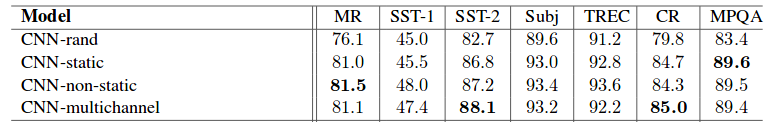
\includegraphics[width=.95\textwidth]{figure/kim}};
\node [red] at (-2,0.25) {\tiny (randomly initialized)};
\node [red] at (-1.95,-0.05) {\tiny (pretrained+frozen)};
\node [red] at (-2.1,-0.35) {\tiny (pretrained+fine-tuned)};
\node [red] at (-1.7,-0.65) {\tiny (combination)};
\end{tikzpicture}

Table from Kim 2014: Convolutional Neural Networks for Sentence Classification.

\vfill

\end{vbframe}

% ------------------------------------------------------------------------------

\begin{vbframe}{Resources}

\vfill

\begin{itemize}
	\item \url{https://fasttext.cc/docs/en/crawl-vectors.html}
		\begin{itemize}
			\item Embeddings for 157 languages, trained on big web crawls, up to 2M words per language
		\end{itemize}
	\item \url{https://nlp.stanford.edu/projects/glove/}
		\begin{itemize}
			\item GloVe word vectors: Co-occurrence-count objective, not n-gram based
		\end{itemize}
\end{itemize}

\vfill

\end{vbframe}

% ------------------------------------------------------------------------------

\begin{vbframe}{Analogy Mining (1)}

\vfill

\textbf{country-capital}
$$\vec w^{(\text{Tokio})} - \vec w^{(\text{Japan})} +  \vec w^{(\text{Poland})} \approx \vec w^{(\text{Warsaw})}$$
\textbf{opposite}
$$\vec w^{(\text{unacceptable})} - \vec w^{(\text{acceptable})} +  \vec w^{(\text{logical})} \approx \vec w^{(\text{illogical})}$$
\textbf{Nationality-adjective}
$$\vec w^{(\text{Australian})} - \vec w^{(\text{Australia})} +  \vec w^{(\text{Switzerland})} \approx \vec w^{(\text{Swiss})}$$

\vfill

\end{vbframe}

% ------------------------------------------------------------------------------

\begin{vbframe}{Analogy Mining (2)}

\begin{center}
\begin{tikzpicture}
\node at (0,0) {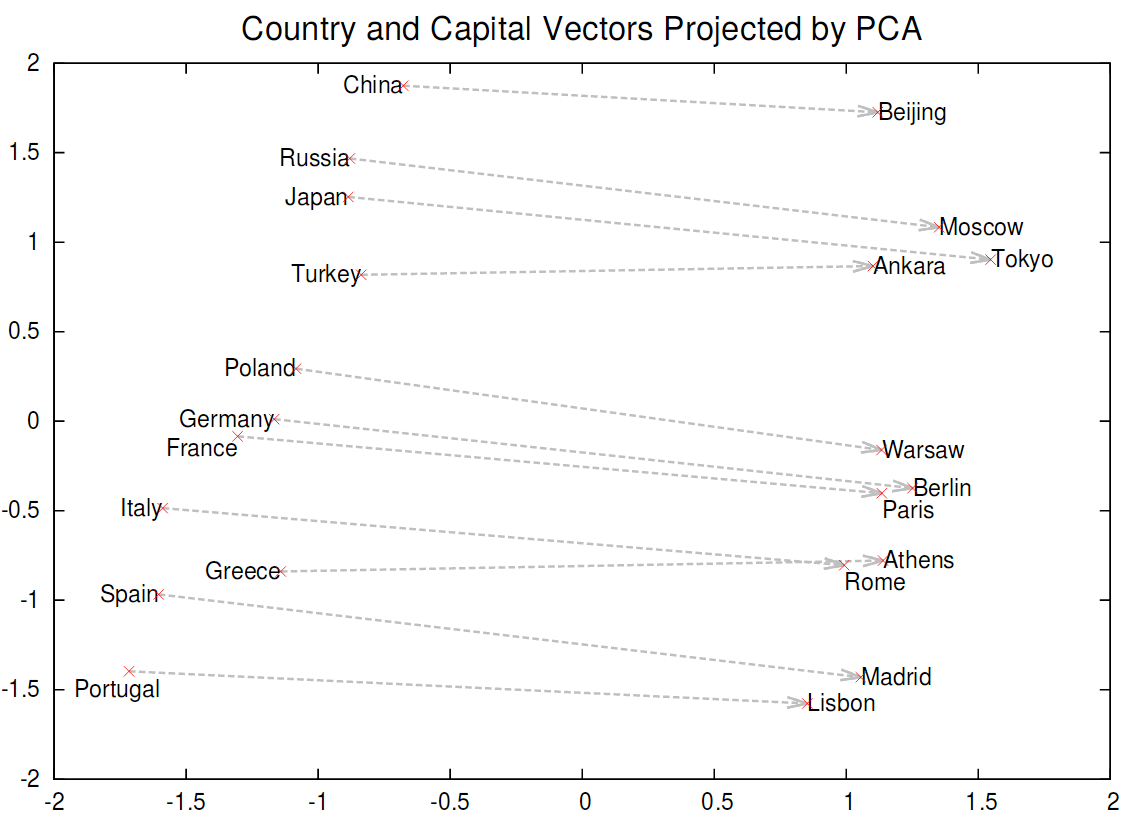
\includegraphics[width = 0.82\textwidth]{figure/countries_capitals}};
\draw [->, thick] (0.2,-0.2) -- (4.1,1.5);
\draw [->, thick] (0.2,-0.2) -- (-2.1,2);
\draw [->, thick] (0.2,-0.2) -- (-2.6,0.45);
\draw [->, thick, red] (4.1,1.5) -- (6.4,-0.7);
\draw [->, thick, green] (6.4,-0.7) -- (3.6, -0.05);
\end{tikzpicture}
\end{center}

\end{vbframe}

% ------------------------------------------------------------------------------

\begin{vbframe}{Analogy Mining (3)}

\vfill

\begin{center}
$$\vec w^{(a)} - \vec w^{(b)} +  \vec w^{(c)} = \vec w^{(?)}$$
$$\vec w^{(d)} = \underset{\vec w^{(d')} \in \mathbf{W}}{\mathrm{argmax}} \quad \mathrm{cos}(\vec w^{(?)}, \vec w^{(d')})$$
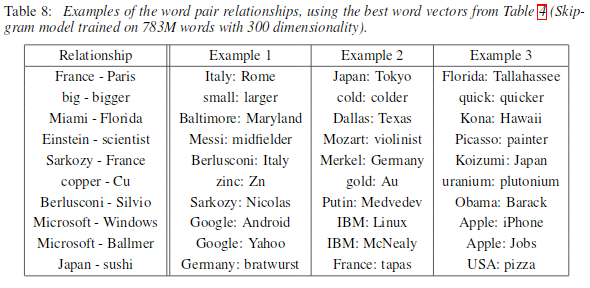
\includegraphics[width = 0.9\textwidth]{figure/similar_relationships}
\end{center}

\vfill

\end{vbframe}

% ------------------------------------------------------------------------------

\begin{vbframe}{Summary}

\vfill

\begin{itemize}
	\item Applications of Word Embeddings
		\begin{itemize}
			\item Word vector initialization in neural networks for NLP tasks
				\begin{itemize}
					\item E.g., sentiment classification of reviews, topical classification of news 
				\end{itemize}
			\item Analogy mining
			\item Information retrieval: semantic search, query expansion
			\item Simple and fast aggregations of sentence representations
			\item \dots
		\end{itemize}
	%\item Word translation mining
	\item Any questions...?
\end{itemize}

\vfill

\end{vbframe}

% ------------------------------------------------------------------------------

\endlecture
\end{document}
